%!TEX root = bambi-thesis.tex

\chapter{Mavros} % (fold)
\label{appendix:mavros}
Mavros package implements a MAVLink extendable communication node for ROS with UDP proxy for Ground Control Station that includes the following features:
\begin{itemize}
	\item Communication with autopilot via serial port
	\item UDP proxy for Ground Control Station
	\item Plugin system for ROS-MAVLink translation
	\item Parameter manipulation tool
	\item Waypoint manipulation tool'
\end{itemize}

 \begin{figure}[ht]
    \centering
    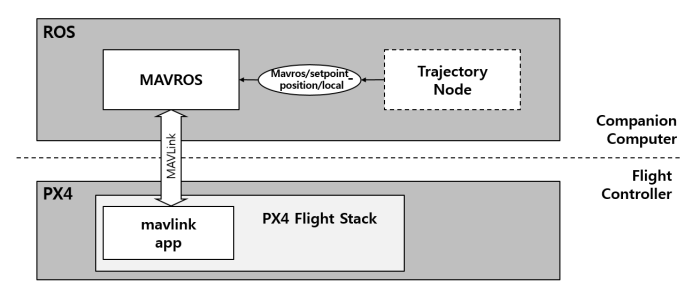
\includegraphics[width=.7\textwidth]{figures/A4/diagram.png}
    \caption{Mavros as communication gateway}
    \label{fig:mavros-diagram}
\end{figure}
Through mavros it is possible to communicate with the flight controller (\autoref{fig:mavros-diagram}) simply publishing over the topic subscribed by mavros or making a call to the services it provides.
The package is made up of various plugins, each handling different components of the FCU.
Every plugin can be load and configure separately when starting mavros through \textit{launch} file. Inside the package there are already some sample launch files specifically created to configure the communication with PX4 or APM flight stack.

% chapter mavros (end)